% -*- coding: utf-8 -*-
\section{Solvation Effects in Quantum Chemistry}

Although all previous sections have modelled chemical systems in a
non-interacting framework ---completely isolated from the rest of the
universe--- this picture fails to reflect the actual conditions under which
most chemical phenomena occur. With the exception of solid-state and
astrochemistry, most chemical reactions and experimental structure
determinations are carried out in solution. On the contrary, standard quantum
chemical calculations often treat isolated molecular species in the gas phase.
This mismatch between theoretical models and experimental conditions can lead
to significant discrepancies in predicted reactivity, stability, and mechanism.

A classic example of this is the addition of bromine to an ethylenic
hydrocarbon, a reaction whose mechanism is known to differ between gas-phase
and solution-phase conditions. Even when the mechanism remains unchanged, the
kinetic behaviour can vary dramatically: for instance, the rate constant for
bromination may differ by a factor of $10^{10}$ when switching from carbon
tetrachloride to water as solvent~\cite{Monard2017, Reichardt1979}.

Numerous strategies have been developed to incorporate solvation effects into
quantum chemical calculations. Broadly, these approaches fall into two
categories: $i$) \emph{explicit} and $ii$) \emph{implicit} solvation models. Explicit
models treat solvent molecules individually, placing them around the solute to
allow direct solute-solvent interactions to be sampled, typically via molecular
dynamics or Monte Carlo simulations. In contrast, implicit models replace the
discrete solvent with a continuous medium characterised by bulk
properties such as the dielectric constant. These continuum approaches are
generally less computationally demanding and are especially well-suited to
routine quantum chemical workflows.

\newpage
\subsection{The Continuum Solvation Model}

A basic continuum model relies on several idealised assumptions:
$i$) the solute is treated at a uniform quantum mechanical level,
$ii$) solute-solvent interactions are limited to electrostatic effects,
$iii$) the system represents a very dilute solution,
$iv$) the solvent is isotropic,
$v$) only the electronic ground state of the solute is considered, and
$vi$) dynamic effects (\eg, solvent relaxation) are neglected~\cite{Tomasi2005}.

An early attempt to estimate the electrostatic contribution to the free energy
of solvation was due to Kirkwood~\cite{Kirkwood1934}, who proposed a model based on a
multipole expansion of the solute charge distribution centred within a spherical
cavity surrounded by a dielectric continuum representing the solvent.

\begin{wrapfigure}[11]{r}{0.50\textwidth}
  \centering
  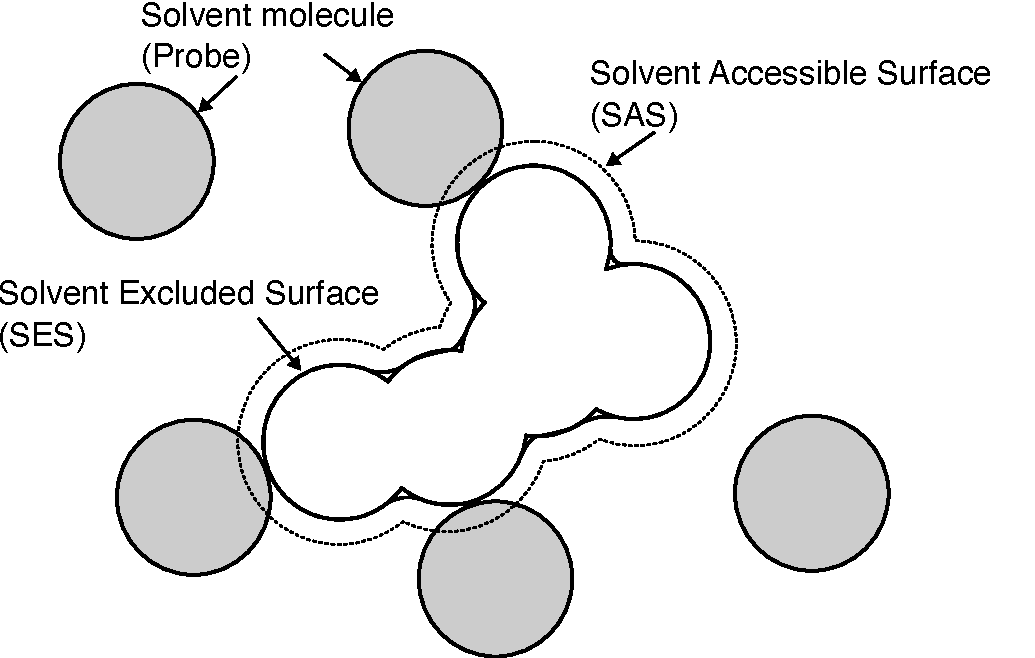
\includegraphics[width=0.48\textwidth]{img/cavity.pdf}
  \caption{Solvent accessible surface (SAS) traced out by
    the center of the probe representing a solvent molecule.
    The solvent excluded surface (SES) is the topological
    boundary of the union of all possible probes that do not
    overlap with the molecule.}
  \label{cavity}
\end{wrapfigure}

A key concept in all continuum models is the cavity (illustrated in
Figure~\ref{cavity}) in which the solute is embedded. This cavity defines a
void region within the continuous dielectric medium, intended to mimic the
exclusion of solvent molecules from the solute volume. The shape and size of
this cavity vary among different continuum models, but it should ideally
exclude solvent penetration while containing the largest possible fraction of
the solute's electron density~\cite{Tomasi2000}. The optimal cavity definition
has been a topic of considerable discussion, and various schemes have been
proposed, typically based on atom-specific radii or electron density
isosurfaces.

The cavity is often defined using concepts such as the solvent-accessible
surface (SAS) and the solvent-excluding surface (SES), which aim to account for 
the physical space inaccessible to solvent molecules due to the 
three-dimensional shape of the solute. The SES, also known as the Connolly
surface, is constructed by rolling a spherical probe (representing a solvent
molecule) over the van der Waals surface of the solute.

\newpage
This results in a composite surface comprising convex, toroidal, and concave
(reentrant) regions, depending on whether the probe is in contact with one,
two, or three atomic spheres, respectively. Analytical representations of the
SES, first developed by Connolly~\cite{Connolly1983}, remain widely used,
although they present computational challenges, such as the treatment of
singularities and cusps.

Computational implementations, such as MSMS~\cite{Sanner1996}, have improved
the stability and triangulation of these surfaces, making them suitable for
applications in continuum solvation models. While detailed surface construction
is rarely necessary for all solvation methods, the SES concept remains
fundamental in defining realistic molecular cavities that exclude solvent
penetration.

\subsection{COSMO: Conductor-like Screening Model}

The COSMO model is a dielectric continuum approach in which the solute is embedded
within a molecule-shaped cavity surrounded by a dielectric medium characterised by
a given dielectric constant $\epsilon$. Electrostatic interactions are first computed
under the assumption that the surrounding medium behaves as a perfect conductor
($\epsilon = \infty$), and are subsequently scaled to reflect the properties of the
actual solvent.

Originally introduced by Klamt and Schüürmann~\cite{Klamt1993}, this method
simplifies the solution of the electrostatic boundary problem. In the idealised
case of a conductor, the total electrostatic potential vanishes at the surface
of the cavity, which allows for an efficient determination of the induced
surface charge distribution.  To recover the correct behaviour for media with
finite $\epsilon$, the idealised surface charge density $\sigma^*(s)$
---obtained under the conductor assumption--- is scaled according to:
$\sigma(s) = f(\epsilon) \, \sigma^*(s)$, where $s$ denotes a point on the
cavity surface, and $f(\epsilon)$ is an empirical scaling function determined
by comparison to accurate solute-solvent electrostatic energies,
given by:
%
\begin{align}
  f(\epsilon) = \frac{\epsilon - 1}{\epsilon + k},
\end{align}
%
\noindent where the empirical parameter $k$ is typically set to a value between
0.5 and 1.0, depending on the implementation. In \adf, for example,
the default atomic cavity radii are taken from the Van der Waals radii of
the MM3 force field, scaled by a factor of 1.2~\cite{Allinger1994, adfcosmo}.

It is important to note that the correction introduced by this factor is
relatively small for solvents with a high dielectric constant, and the final
solvation energy is generally insensitive to variations in the $k$ parameter~\cite{Tomasi2005}.

The inclusion of a linear parametrisation of non-electrostatic contributions is
also possible as a function of surface area, introducing a correction that
accounts for dispersion and cavity formation effects. Typically, only the
surface area-dependent term is retained. This leads to the following
expression:

\begin{align}
  E_\text{non-elec} = f(\epsilon)\left(Cav_0 + Cav_1\times\text{area}\right).
\end{align}

\subsection{The Quantum Mechanical/Molecular Mechanical (QM/MM) Models}

In many chemical systems, the solvent acts primarily as a physical
perturbation on a solute of interest (an individual molecule, a
molecular complex, or a transition state)~\cite{Monard2017}. This separation of
roles allows the chemically relevant subsystem to be treated at a higher level
of theory, while the surrounding environment is described at a lower, less
computationally demanding level.

Hybrid quantum mechanical/molecular mechanical (QM/MM) models take advantage of
this partitioning. In these approaches, the solute is treated using quantum
chemical methods, while the solvent is represented by a classical force field.
The total Hamiltonian of the system is expressed as the sum of three
contributions~\cite{Monard2003}:
%
\begin{align}
  \Ha_\text{QM/MM} = \Ha_\text{QM} + \Ha_\text{MM} + \Ha_\text{QM/MM},
\end{align}

\noindent the first term is the quantum mechanical Hamiltonian of the solute, and the
second is the classical Hamiltonian that describes the configuration of the
solvent. Both are well-defined by the chosen quantum mechanical methodology and
classical force field, respectively. The third term, which represents the
interaction between the quantum solute and classical solvent, can be
implemented in various ways.

\newpage
One common approach includes: $i$) Van der Waals interactions between classical
solvent atoms and quantum solute atoms; $ii$) long-range electrostatic
interactions among the classical solvent molecules; and $iii$) the interaction
between the electron density and nuclei of the solute and the classical
solvent, which may also involve specific interactions such as hydrogen
bonding~\cite{Monard2017}.

Polarisable Embedding (PE) models extend this framework by introducing the
self-energy of induced dipoles ---representing the work required to induce the
dipoles themselves--- and the mutual repulsion between all induced dipoles. These
contributions appear as the third and fourth terms in the following expression:

\begin{align}
  E^\text{QM/MM} =&\, \sfrac{1}{2}\sum_iq_iV_i^\text{MM} + \sum_iq_iV_i^\text{QM}
    + \sfrac{1}{2}\,\sum_i \left(\alpha_i^{-1}\mu_i^2 +
      \sum_{j\neq i}\mu_i\mathscr{T}_{ij}\mu_j\right) \nonumber\\
    &- \sum_i\mu_i \left(E_i^\text{MM} + E_i^\text{QM}\right),
\end{align}

\noindent where $\mathscr{T}_{ij}$ denotes the effective dipole-field
interaction tensor~\cite{Lipparini2014, Bondanza2020}, which introduces
distance dependent damping functions to avoid the divergence of the Coulomb
interaction between two point dipoles when they get too
close~\cite{Ponder2003}.

